\documentclass{standalone}
\usepackage{tikz}
\usetikzlibrary{patterns, positioning}


\begin{document}
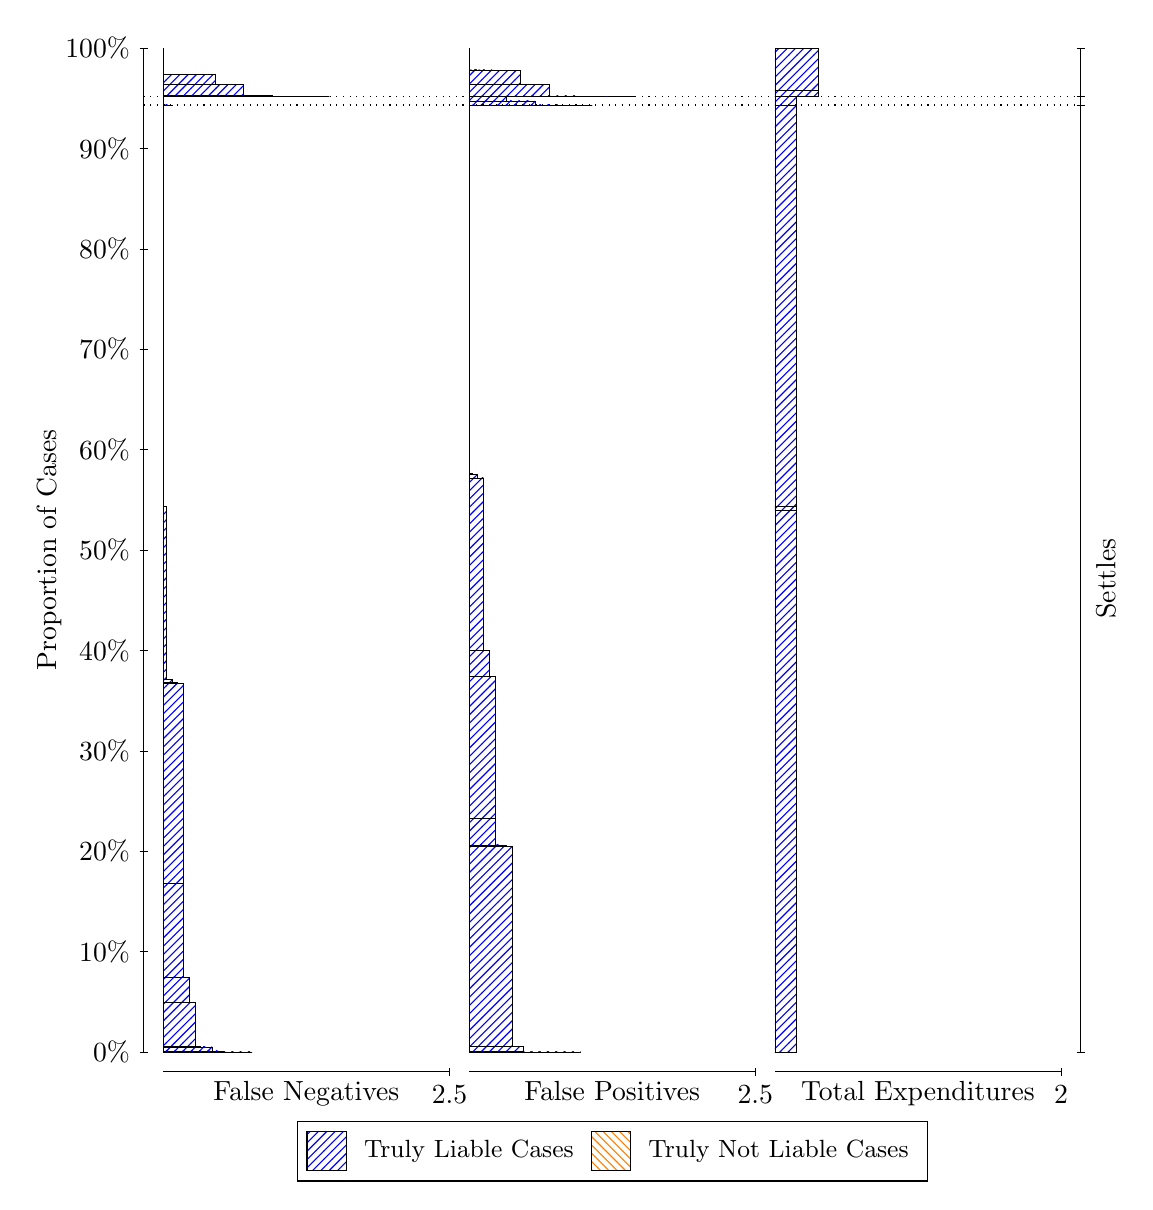
\begin{tikzpicture}
\draw[black, very thin] (1.5,1.75) -- (1.5,14.5);
\node[rotate=90, text=black, anchor=center] at (0.3, 8.125) {Proportion of Cases};
\draw[black, very thin] (1.45,1.75) -- (1.55,1.75);
\node[text=black, anchor=east] at (1.45, 1.75) {0\%};
\draw[black, very thin] (1.45,3.025) -- (1.55,3.025);
\node[text=black, anchor=east] at (1.45, 3.025) {10\%};
\draw[black, very thin] (1.45,4.3) -- (1.55,4.3);
\node[text=black, anchor=east] at (1.45, 4.3) {20\%};
\draw[black, very thin] (1.45,5.575) -- (1.55,5.575);
\node[text=black, anchor=east] at (1.45, 5.575) {30\%};
\draw[black, very thin] (1.45,6.85) -- (1.55,6.85);
\node[text=black, anchor=east] at (1.45, 6.85) {40\%};
\draw[black, very thin] (1.45,8.125) -- (1.55,8.125);
\node[text=black, anchor=east] at (1.45, 8.125) {50\%};
\draw[black, very thin] (1.45,9.4) -- (1.55,9.4);
\node[text=black, anchor=east] at (1.45, 9.4) {60\%};
\draw[black, very thin] (1.45,10.675) -- (1.55,10.675);
\node[text=black, anchor=east] at (1.45, 10.675) {70\%};
\draw[black, very thin] (1.45,11.95) -- (1.55,11.95);
\node[text=black, anchor=east] at (1.45, 11.95) {80\%};
\draw[black, very thin] (1.45,13.225) -- (1.55,13.225);
\node[text=black, anchor=east] at (1.45, 13.225) {90\%};
\draw[black, very thin] (1.45,14.5) -- (1.55,14.5);
\node[text=black, anchor=east] at (1.45, 14.5) {100\%};

\draw[black, very thin] (13.4,1.75) -- (13.4,14.5);
\draw[black, very thin] (13.35,1.75) -- (13.45,1.75);
\node[anchor=west] at (13.35, 1.75) {};
\draw[black, very thin] (13.35,13.776) -- (13.45,13.776);
\node[anchor=west] at (13.35, 13.776) {};
\draw[black, very thin] (13.35,13.886) -- (13.45,13.886);
\node[anchor=west] at (13.35, 13.886) {};
\draw[black, very thin] (13.35,14.5) -- (13.45,14.5);
\node[anchor=west] at (13.35, 14.5) {};

\draw[black, very thin, pattern color=blue, pattern=north east lines] (1.75,1.75) rectangle (2.8763,1.75);
\draw[black, very thin, pattern color=blue, pattern=north east lines] (1.75,1.75) rectangle (2.731,1.75);
\draw[black, very thin, pattern color=blue, pattern=north east lines] (1.75,1.75) rectangle (2.5857,1.75);
\draw[black, very thin, pattern color=blue, pattern=north east lines] (1.75,1.75) rectangle (2.513,1.7605);
\draw[black, very thin, pattern color=blue, pattern=north east lines] (1.75,1.7605) rectangle (2.4403,1.7644);
\draw[black, very thin, pattern color=blue, pattern=north east lines] (1.75,1.7644) rectangle (2.3677,1.8156);
\draw[black, very thin, pattern color=blue, pattern=north east lines] (1.75,1.8156) rectangle (2.295,1.8157);
\draw[black, very thin, pattern color=blue, pattern=north east lines] (1.75,1.8157) rectangle (2.2223,1.818);
\draw[black, very thin, pattern color=blue, pattern=north east lines] (1.75,1.818) rectangle (2.1497,2.3765);
\draw[black, very thin, pattern color=blue, pattern=north east lines] (1.75,2.3765) rectangle (2.077,2.7029);
\draw[black, very thin, pattern color=blue, pattern=north east lines] (1.75,2.7029) rectangle (2.0043,3.8874);
\draw[black, very thin, pattern color=blue, pattern=north east lines] (1.75,3.8874) rectangle (2.0043,6.4292);
\draw[black, very thin, pattern color=blue, pattern=north east lines] (1.75,6.4292) rectangle (1.9317,6.4435);
\draw[black, very thin, pattern color=blue, pattern=north east lines] (1.75,6.4435) rectangle (1.859,6.4857);
\draw[black, very thin, pattern color=blue, pattern=north east lines] (1.75,6.4857) rectangle (1.7863,8.6781);
\draw[black, very thin, pattern color=orange, pattern=north west lines] (1.75,8.6781) rectangle (1.75,8.6781);
\draw[black, very thin, pattern color=blue, pattern=north east lines] (1.75,8.6781) rectangle (1.75,13.776);
\draw[black, very thin, pattern color=blue, pattern=north east lines] (1.75,13.776) rectangle (1.859,13.777);
\draw[black, very thin, pattern color=orange, pattern=north west lines] (1.75,13.777) rectangle (1.75,13.777);
\draw[black, very thin, pattern color=blue, pattern=north east lines] (1.75,13.777) rectangle (1.75,13.886);
\draw[black, very thin, pattern color=blue, pattern=north east lines] (1.75,13.886) rectangle (3.8573,13.886);
\draw[black, very thin, pattern color=blue, pattern=north east lines] (1.75,13.886) rectangle (3.494,13.886);
\draw[black, very thin, pattern color=blue, pattern=north east lines] (1.75,13.886) rectangle (3.1307,13.899);
\draw[black, very thin, pattern color=blue, pattern=north east lines] (1.75,13.899) rectangle (2.7673,14.041);
\draw[black, very thin, pattern color=blue, pattern=north east lines] (1.75,14.041) rectangle (2.404,14.164);
\draw[black, very thin, pattern color=blue, pattern=north east lines] (1.75,14.164) rectangle (2.2587,14.164);
\draw[black, very thin, pattern color=blue, pattern=north east lines] (1.75,14.164) rectangle (2.0407,14.164);
\draw[black, very thin, pattern color=blue, pattern=north east lines] (1.75,14.164) rectangle (1.8953,14.166);
\draw[black, very thin, pattern color=orange, pattern=north west lines] (1.75,14.166) rectangle (1.75,14.166);
\draw[black, very thin, pattern color=blue, pattern=north east lines] (1.75,14.166) rectangle (1.75,14.5);
\draw[black, very thin, pattern color=orange, pattern=north west lines] (5.6333,1.75) rectangle (7.0503,1.75);
\draw[black, very thin, pattern color=blue, pattern=north east lines] (5.6333,1.75) rectangle (7.0503,1.75);
\draw[black, very thin, pattern color=orange, pattern=north west lines] (5.6333,1.75) rectangle (6.7597,1.75);
\draw[black, very thin, pattern color=blue, pattern=north east lines] (5.6333,1.75) rectangle (6.7597,1.75);
\draw[black, very thin, pattern color=blue, pattern=north east lines] (5.6333,1.75) rectangle (6.687,1.75);
\draw[black, very thin, pattern color=orange, pattern=north west lines] (5.6333,1.75) rectangle (6.6143,1.75);
\draw[black, very thin, pattern color=blue, pattern=north east lines] (5.6333,1.75) rectangle (6.6143,1.75);
\draw[black, very thin, pattern color=orange, pattern=north west lines] (5.6333,1.75) rectangle (6.469,1.75);
\draw[black, very thin, pattern color=blue, pattern=north east lines] (5.6333,1.75) rectangle (6.469,1.75);
\draw[black, very thin, pattern color=blue, pattern=north east lines] (5.6333,1.75) rectangle (6.3963,1.75);
\draw[black, very thin, pattern color=orange, pattern=north west lines] (5.6333,1.75) rectangle (6.3237,1.75);
\draw[black, very thin, pattern color=blue, pattern=north east lines] (5.6333,1.75) rectangle (6.3237,1.7535);
\draw[black, very thin, pattern color=blue, pattern=north east lines] (5.6333,1.7535) rectangle (6.3237,1.8176);
\draw[black, very thin, pattern color=blue, pattern=north east lines] (5.6333,1.8176) rectangle (6.251,1.8211);
\draw[black, very thin, pattern color=orange, pattern=north west lines] (5.6333,1.8211) rectangle (6.1783,1.8211);
\draw[black, very thin, pattern color=blue, pattern=north east lines] (5.6333,1.8211) rectangle (6.1783,4.3675);
\draw[black, very thin, pattern color=blue, pattern=north east lines] (5.6333,4.3675) rectangle (6.1057,4.3697);
\draw[black, very thin, pattern color=blue, pattern=north east lines] (5.6333,4.3697) rectangle (6.033,4.3814);
\draw[black, very thin, pattern color=blue, pattern=north east lines] (5.6333,4.3814) rectangle (5.9603,4.7151);
\draw[black, very thin, pattern color=blue, pattern=north east lines] (5.6333,4.7151) rectangle (5.9603,6.5192);
\draw[black, very thin, pattern color=blue, pattern=north east lines] (5.6333,6.5192) rectangle (5.8877,6.8479);
\draw[black, very thin, pattern color=blue, pattern=north east lines] (5.6333,6.8479) rectangle (5.815,9.0404);
\draw[black, very thin, pattern color=blue, pattern=north east lines] (5.6333,9.0404) rectangle (5.7423,9.0826);
\draw[black, very thin, pattern color=blue, pattern=north east lines] (5.6333,9.0826) rectangle (5.6697,9.0969);
\draw[black, very thin, pattern color=blue, pattern=north east lines] (5.6333,9.0969) rectangle (5.6333,13.776);
\draw[black, very thin, pattern color=orange, pattern=north west lines] (5.6333,13.776) rectangle (7.1957,13.776);
\draw[black, very thin, pattern color=blue, pattern=north east lines] (5.6333,13.776) rectangle (7.1957,13.776);
\draw[black, very thin, pattern color=blue, pattern=north east lines] (5.6333,13.776) rectangle (6.8323,13.777);
\draw[black, very thin, pattern color=blue, pattern=north east lines] (5.6333,13.777) rectangle (6.469,13.83);
\draw[black, very thin, pattern color=blue, pattern=north east lines] (5.6333,13.83) rectangle (6.1057,13.885);
\draw[black, very thin, pattern color=blue, pattern=north east lines] (5.6333,13.885) rectangle (5.7423,13.886);
\draw[black, very thin, pattern color=orange, pattern=north west lines] (5.6333,13.886) rectangle (7.7407,13.886);
\draw[black, very thin, pattern color=blue, pattern=north east lines] (5.6333,13.886) rectangle (7.7407,13.886);
\draw[black, very thin, pattern color=orange, pattern=north west lines] (5.6333,13.886) rectangle (7.3773,13.886);
\draw[black, very thin, pattern color=blue, pattern=north east lines] (5.6333,13.886) rectangle (7.3773,13.886);
\draw[black, very thin, pattern color=orange, pattern=north west lines] (5.6333,13.886) rectangle (7.014,13.886);
\draw[black, very thin, pattern color=blue, pattern=north east lines] (5.6333,13.886) rectangle (7.014,13.893);
\draw[black, very thin, pattern color=blue, pattern=north east lines] (5.6333,13.893) rectangle (6.6507,14.035);
\draw[black, very thin, pattern color=blue, pattern=north east lines] (5.6333,14.035) rectangle (6.2873,14.219);
\draw[black, very thin, pattern color=orange, pattern=north west lines] (5.6333,14.219) rectangle (6.142,14.219);
\draw[black, very thin, pattern color=blue, pattern=north east lines] (5.6333,14.219) rectangle (6.142,14.219);
\draw[black, very thin, pattern color=blue, pattern=north east lines] (5.6333,14.219) rectangle (5.924,14.221);
\draw[black, very thin, pattern color=orange, pattern=north west lines] (5.6333,14.221) rectangle (5.7787,14.221);
\draw[black, very thin, pattern color=blue, pattern=north east lines] (5.6333,14.221) rectangle (5.7787,14.221);
\draw[black, very thin, pattern color=blue, pattern=north east lines] (5.6333,14.221) rectangle (5.7787,14.221);
\draw[black, very thin, pattern color=orange, pattern=north west lines] (5.6333,14.221) rectangle (5.6333,14.221);
\draw[black, very thin, pattern color=blue, pattern=north east lines] (5.6333,14.221) rectangle (5.6333,14.5);
\draw[black, very thin, pattern color=orange, pattern=north west lines] (9.5167,1.75) rectangle (9.7892,1.75);
\draw[black, very thin, pattern color=blue, pattern=north east lines] (9.5167,1.75) rectangle (9.7892,8.6306);
\draw[black, very thin, pattern color=orange, pattern=north west lines] (9.5167,8.6306) rectangle (9.7892,8.6306);
\draw[black, very thin, pattern color=blue, pattern=north east lines] (9.5167,8.6306) rectangle (9.7892,8.6773);
\draw[black, very thin, pattern color=orange, pattern=north west lines] (9.5167,8.6773) rectangle (9.7892,8.6773);
\draw[black, very thin, pattern color=blue, pattern=north east lines] (9.5167,8.6773) rectangle (9.7892,13.776);
\draw[black, very thin, pattern color=orange, pattern=north west lines] (9.5167,13.776) rectangle (9.7892,13.776);
\draw[black, very thin, pattern color=blue, pattern=north east lines] (9.5167,13.776) rectangle (9.7892,13.886);
\draw[black, very thin, pattern color=orange, pattern=north west lines] (9.5167,13.886) rectangle (10.062,13.886);
\draw[black, very thin, pattern color=blue, pattern=north east lines] (9.5167,13.886) rectangle (10.062,13.962);
\draw[black, very thin, pattern color=orange, pattern=north west lines] (9.5167,13.962) rectangle (10.062,13.962);
\draw[black, very thin, pattern color=blue, pattern=north east lines] (9.5167,13.962) rectangle (10.062,14.5);
\draw[black, dotted] (1.5,13.776) -- (13.4,13.776);
\draw[black, dotted] (1.5,13.886) -- (13.4,13.886);
\draw[black, very thin] (1.75,1.5) -- (5.3833,1.5);
\node[text=black, anchor=north] at (3.5667, 1.5) {False Negatives};
\draw[black, very thin] (5.3833,1.45) -- (5.3833,1.55);
\node[text=black, anchor=north] at (5.3833, 1.45) {2.5};

\draw[black, very thin] (5.6333,1.5) -- (9.2667,1.5);
\node[text=black, anchor=north] at (7.45, 1.5) {False Positives};
\draw[black, very thin] (9.2667,1.45) -- (9.2667,1.55);
\node[text=black, anchor=north] at (9.2667, 1.45) {2.5};

\draw[black, very thin] (9.5167,1.5) -- (13.15,1.5);
\node[text=black, anchor=north] at (11.333, 1.5) {Total Expenditures};
\draw[black, very thin] (13.15,1.45) -- (13.15,1.55);
\node[text=black, anchor=north] at (13.15, 1.45) {2};

\node[text=black, centered, rotate=90] at (13.72, 7.763) {Settles};



\draw (7.449999999999999,1.5) node[draw=none] (baseCoordinate) {};
\begin{scope}[align=center]
        \matrix[scale=0.5, draw=black, below=0.5cm of baseCoordinate, nodes={draw}, column sep=0.1cm]{
            \node[rectangle, draw, minimum width=0.5cm, minimum height=0.5cm, pattern color=blue, pattern=north east lines] {}; &
            \node[draw=none, font=\small, text=black] (B) {Truly Liable Cases}; &
            \node[rectangle, draw, minimum width=0.5cm, minimum height=0.5cm, pattern color=orange, pattern=north west lines] {}; &
            \node[draw=none, font=\small, text=black] (B) {Truly Not Liable Cases}; \\
            };
\end{scope}

\end{tikzpicture}
\end{document}